\section*{Conceptual Framework}
\subsection*{Positioning the Concept of the Ideational Bricoleur}

In order to clarify the conceptual contribution, the notion of the 
\textit{ideational bricoleur} must be situated against established approaches to 
agency in policy and governance. First, \textit{policy entrepreneurs}, in 
Kingdon’s multiple streams framework, are defined by their ability to exploit 
windows of opportunity and to couple problem, policy, and political streams. 
Their focus lies on timing and agenda access. Second, Hajer’s 
\textit{discourse coalition brokers} emphasize the role of actors in weaving 
storylines across networks, thereby enabling coalitions to stabilize 
interpretations of complex environmental problems. By contrast, the 
\textit{ideational bricoleur} highlights a different dimension of agency: the 
substantive recombination of discursive elements and institutional instruments. 
Rather than coupling streams or narrating storylines, the ideational bricoleur 
assembles heterogeneous fragments---scientific claims, legal tools, economic 
incentives, customary practices---into novel governance proposals. This 
analytical lens reveals how adaptation strategies are not merely adopted from 
pre-existing repertoires but crafted through a pragmatic patchwork of ideas and 
institutions. In this sense, the concept complements discursive institutionalism 
by identifying the micro-level practices through which actors mobilize ideational 
power ``in, through, and over ideas'' to construct new logics of governance.

%\begin{figure}[h!]
%\centering
%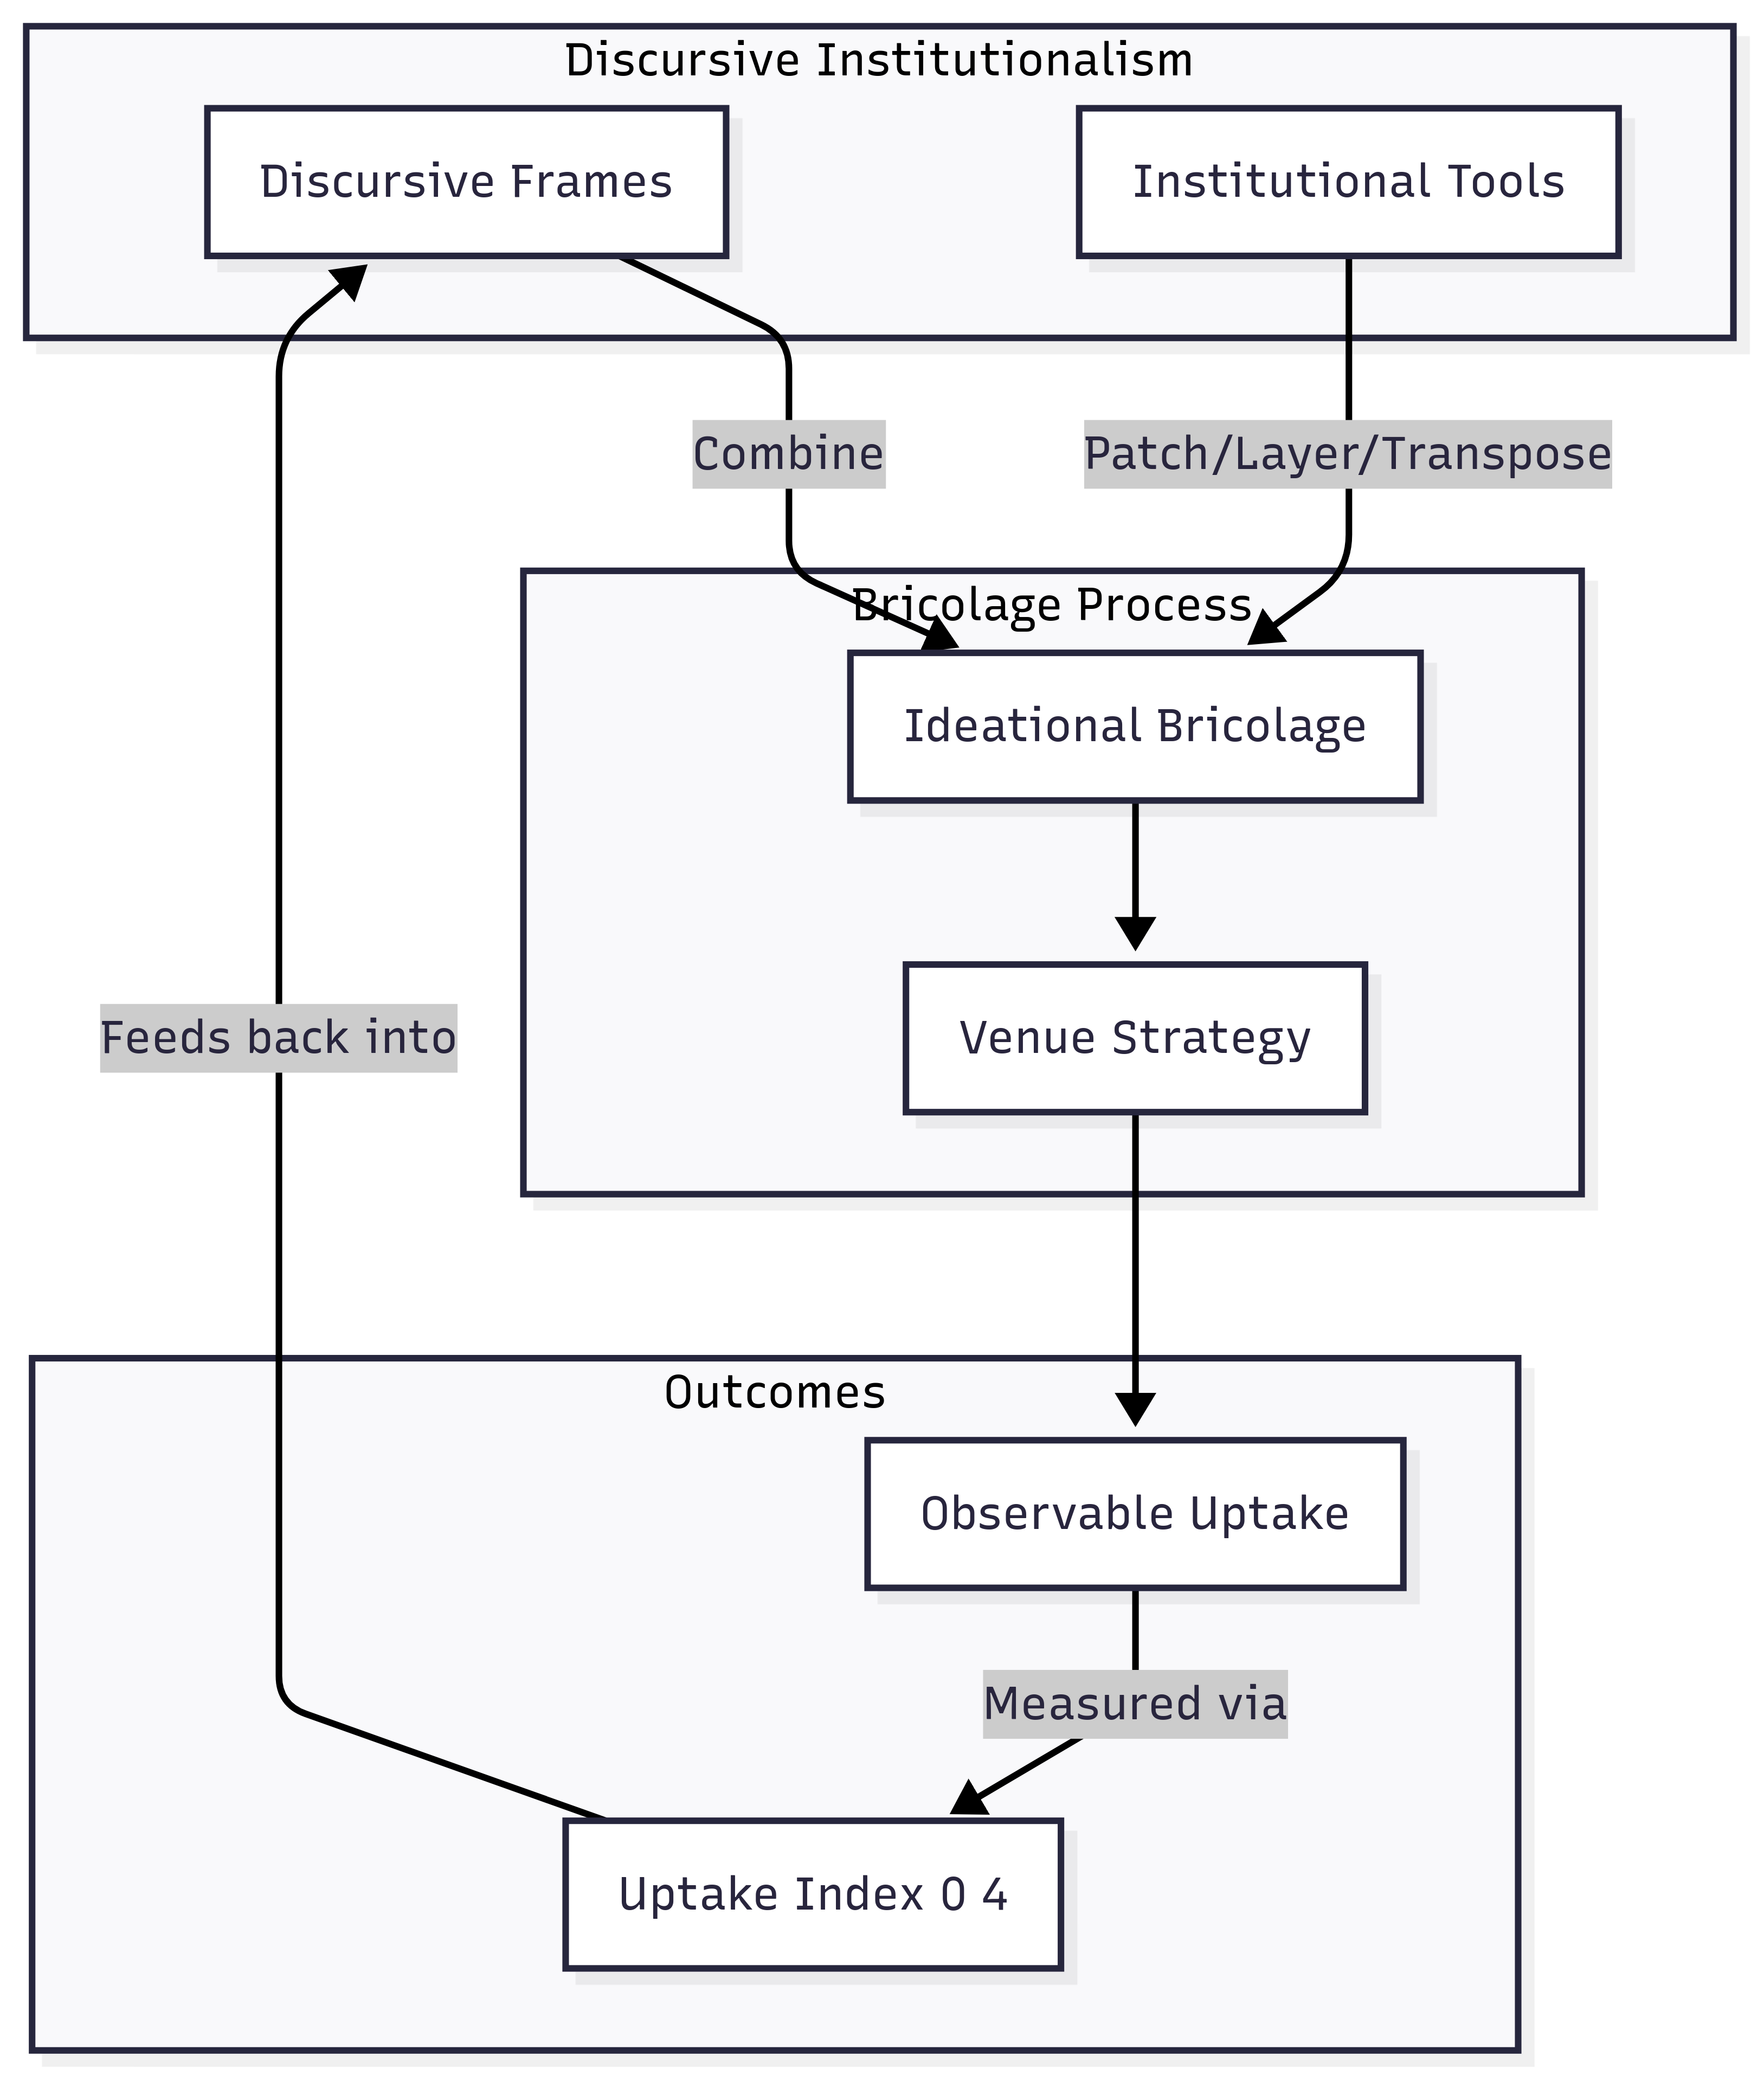
\includegraphics[width=0.8\textwidth]{src/fig/d-inst.png}
%\caption{Discursive Institutionalism}
%\label{fig:prisma-flow}
%\end{figure}


